\documentclass[12pt]{article}%
\usepackage{tikz}
\usepackage{latexsym, amsmath,amsfonts,amssymb}
\usepackage{xcolor}
\usepackage[margin=.75in]{geometry}
\pagestyle{empty}
\begin{document}

\begin{center}
\Large{\textbf{Japanese Line Functions (Amidakuji)}}
\end{center}
They're known as Amidakuji, Ghost Leg, Japanese Ladder Games, 
ladders, and maybe some other names, too. At the time I couldn't
find them on the internet and ended up calling them Japanese 
line functions. Whatever you decide to call it, to create one you'll
draw a finite number of vertical lines followed by 
a finite number of horizontal lines drawn according to these rules:

\begin{enumerate}
	\item A horizontal line starts at one vertical line and ends 
	at the next vertical line.
	\item Horizontal lines never connect the endpoints of the vertical lines.
\end{enumerate}
Finally label top the top and bottom of each vertical line with 
different letters or numbers.

The figure below gives an example made up of 4 vertical lines 
where the rules have been followed correctly and an example 
where the rules have been violated. The 3 errors are in red:
the horizontal line from $b$ to $d$ violates the first rule and 
the lines from $a$ to $b$ and $c$ to $d$ violate the second rule.
\begin{figure}[h!]
\begin{minipage}{.6\textwidth}
\begin{center}
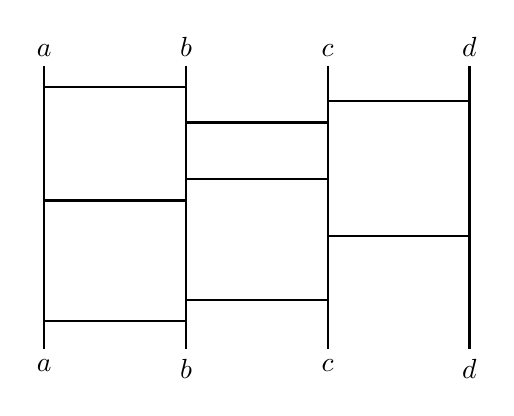
\begin{tikzpicture}[scale=.9]
\foreach \x in {0, ...,3}{
\draw[thick] (2*\x+1,4)--(2*\x+1,0);
}
\coordinate [label=above:$a$] (a1) at (1,4);
\coordinate [label=below:$a$] (a2) at (1,0);
\coordinate [label=above:$b$] (b1) at (3,4);
\coordinate [label=below:$b$] (b2) at (3,0);
\coordinate [label=above:$c$] (c1) at (5,4);
\coordinate [label=below:$c$] (c2) at (5,0);
\coordinate [label=above:$d$] (d1) at (7,4);
\coordinate [label=below:$d$] (d2) at (7,0);
\draw[thick] (1,3.7)--(3,3.7);
\draw[thick] (1,2.1)--(3,2.1);
\draw[thick] (1,.4)--(3,.4);
\draw[thick] (3,3.2)--(5,3.2);
\draw[thick] (3,2.4)--(5,2.4);
\draw[thick] (3,.7)--(5,.7);
\draw[thick] (5,3.5)--(7,3.5);
\draw[thick] (5,1.6)--(7,1.6);
\end{tikzpicture}
\end{center}
\end{minipage}
\begin{minipage}{.4\textwidth}
\begin{center}
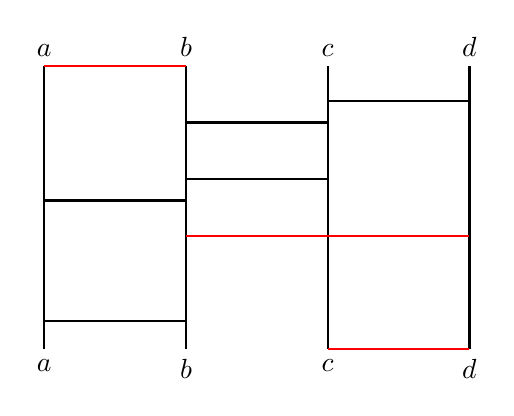
\begin{tikzpicture}[scale=.9]
\foreach \x in {0, ...,3}{
\draw[thick] (2*\x+1,4)--(2*\x+1,0);
}
\coordinate [label=above:$a$] (a1) at (1,4);
\coordinate [label=below:$a$] (a2) at (1,0);
\coordinate [label=above:$b$] (b1) at (3,4);
\coordinate [label=below:$b$] (b2) at (3,0);
\coordinate [label=above:$c$] (c1) at (5,4);
\coordinate [label=below:$c$] (c2) at (5,0);
\coordinate [label=above:$d$] (d1) at (7,4);
\coordinate [label=below:$d$] (d2) at (7,0);
\draw[thick,red] (1,4)--(3,4);
\draw[thick] (1,2.1)--(3,2.1);
\draw[thick] (1,.4)--(3,.4);
\draw[thick] (3,3.2)--(5,3.2);
\draw[thick] (3,2.4)--(5,2.4);
\draw[thick,red] (3,1.6)--(5,1.6);
\draw[thick] (5,3.5)--(7,3.5);
\draw[thick,red] (5,1.6)--(7,1.6);
\draw[thick,red] (5,0)--(7,0);
\end{tikzpicture}
\end{center}
\end{minipage}
\end{figure}

Movement is always on a line according to these rules.
\begin{enumerate}
\item Always move down unless it's possible to move on a line 
left or right.
  \item Moving left or right continues until the next vertical line
 at which point the movement must be down. 
\end{enumerate}
These well defined set of rules ensure that just one 
movement is possible: down, right, or left. 
The path of $a$ has been traced out in the diagram below.
You should confirm that $b$ goes to $c$, $c$ goes to $a$ and $d$
goes to $d$. 
\begin{center}
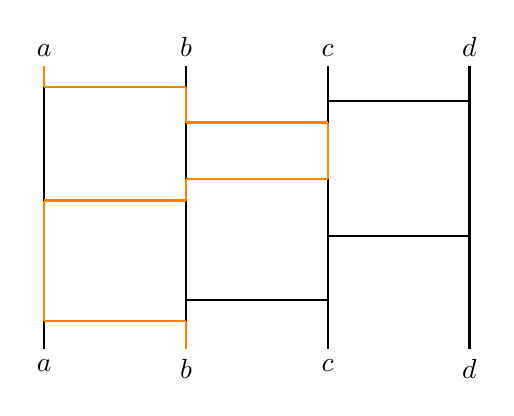
\begin{tikzpicture}[scale=.9]
\foreach \x in {0, ...,3}{
\draw[thick] (2*\x+1,4)--(2*\x+1,0);
}
\coordinate [label=above:$a$] (a1) at (1,4);
\coordinate [label=below:$a$] (a2) at (1,0);
\coordinate [label=above:$b$] (b1) at (3,4);
\coordinate [label=below:$b$] (b2) at (3,0);
\coordinate [label=above:$c$] (c1) at (5,4);
\coordinate [label=below:$c$] (c2) at (5,0);
\coordinate [label=above:$d$] (d1) at (7,4);
\coordinate [label=below:$d$] (d2) at (7,0);
\draw[thick] (1,3.7)--(3,3.7);
\draw[thick] (1,2.1)--(3,2.1);
\draw[thick] (1,.4)--(3,.4);
\draw[thick] (3,3.2)--(5,3.2);
\draw[thick] (3,2.4)--(5,2.4);
\draw[thick] (3,.7)--(5,.7);
\draw[thick] (5,3.5)--(7,3.5);
\draw[thick] (5,1.6)--(7,1.6);
\draw[thick,orange] (1,4)--(1,3.7);
\draw[thick,orange] (1,3.7)--(3,3.7);
\draw[thick,orange] (3,3.7)--(3,3.2);
\draw[thick,orange] (3,3.2)--(5,3.2);
\draw[thick,orange] (5,3.2)--(5,2.4);
\draw[thick,orange] (5,2.4)--(3,2.4);
\draw[thick,orange] (3,2.1)--(3,2.4);
\draw[thick,orange] (3,2.1)--(1,2.1);
\draw[thick,orange] (1,.4)--(1,2.1);
\draw[thick,orange] (1,.4)--(3,.4);
\draw[thick,orange] (3,0)--(3,.4);
\end{tikzpicture}
\end{center}
\end{document}